\documentclass[a4paper,12pt]{article}

\usepackage[utf8]{inputenc}
\usepackage[spanish]{babel}
\usepackage{amsmath, amssymb}
\usepackage{graphicx}
\usepackage{float}
\usepackage{booktabs}
\usepackage{xcolor}
\usepackage{listings}
\usepackage{caption}
\usepackage{fancyhdr}
\usepackage{hyperref}
\usepackage{tikz}

\hypersetup{
    colorlinks=true,
    linkcolor=blue,
    urlcolor=blue,
    pdftitle={Práctica 4 - Sistemas RTOS},
}

% === Definición de colores similares a Vivado ===
\definecolor{vivadoKeyword}{rgb}{0.6,0.0,0.6}
\definecolor{vivadoComment}{rgb}{0.0,0.5,0.0}
\definecolor{vivadoString}{rgb}{0.5,0.2,0.0}
\definecolor{vivadoBackground}{rgb}{0.97,0.97,0.97}

\lstdefinelanguage{VHDL}{
    morekeywords={library, use, entity, is, port, in, out, end, architecture, of, begin, signal, if, then, else, when, others, xor, and, or, not},
    sensitive=true,
    morecomment=[l]--,
    morestring=[b]",
}

\lstset{
    language=VHDL,
    backgroundcolor=\color{vivadoBackground},
    keywordstyle=\color{vivadoKeyword}\bfseries,
    commentstyle=\color{vivadoComment}\itshape,
    stringstyle=\color{vivadoString},
    basicstyle=\ttfamily\small,
    numbers=left,
    numberstyle=\tiny,
    numbersep=5pt,
    frame=single,
    breaklines=true,
    tabsize=2,
    captionpos=b
}

\title{Práctica N°4: Sistemas RTOS}
\date{}

\begin{document}
\maketitle
\tableofcontents
\newpage


\section{Objetivos}

El propósito de esta práctica es introducir al estudiante en el uso de un sistema operativo en tiempo real (RTOS) aplicado al microcontrolador STM32F407, utilizando el entorno de desarrollo STM32CubeIDE y el kernel FreeRTOS. Se busca comprender cómo se gestionan las tareas concurrentes, las prioridades, los retardos y la sincronización mediante interrupciones y semáforos.

\subsection{Objetivo general}

Implementar un sistema multitarea basado en FreeRTOS sobre el microcontrolador STM32F407G-DISC1, que permita ejecutar tareas con distintas prioridades y sincronizar su funcionamiento a través de interrupciones externas, utilizando los mecanismos de planificación y temporización del RTOS.

\subsection{Objetivos específicos}

\begin{itemize}
    \item Comprender la estructura básica de un proyecto con FreeRTOS generado mediante STM32CubeIDE.
    \item Configurar correctamente el kernel de FreeRTOS dentro del entorno STM32CubeMX, habilitando las tareas, prioridades y temporizadores del sistema.
    \item Implementar varias tareas concurrentes con diferentes niveles de prioridad y analizar su comportamiento en ejecución.
    \item Utilizar la comunicación mediante interrupciones externas para modificar el flujo de ejecución de una o más tareas.
    \item Observar el efecto de los retardos (\texttt{osDelay()}) y la planificación por prioridad sobre el tiempo de ejecución de cada tarea.
    \item Consolidar el uso del puerto serie (UART) para la depuración y monitoreo del sistema multitarea.
\end{itemize}

\subsection{Asignación de Pines en el STM32CubeMX}

Una parte fundamental en la configuración de un proyecto en STM32CubeIDE es la asignación de pines dentro del archivo \texttt{.ioc}. Cada periférico del microcontrolador debe conectarse correctamente a los pines físicos de la tarjeta de desarrollo.

En esta práctica se requiere configurar los periféricos del \textbf{UART2}, los \textbf{LEDs integrados} y el \textbf{pulsador de usuario}.

\subsubsection{Pines para los LEDs Integrados}

La tarjeta STM32F407G-DISC1 dispone de cuatro LEDs de usuario conectados al puerto D del microcontrolador. Cada LED puede ser controlado individualmente mediante escritura digital sobre los pines correspondientes:

\begin{itemize}
\item \textbf{PD12}: LED Verde (LD4)
\item \textbf{PD13}: LED Naranja (LD3)
\item \textbf{PD14}: LED Rojo (LD5)
\item \textbf{PD15}: LED Azul (LD6)
\end{itemize}

Cada uno de estos pines debe configurarse como \textbf{GPIO Output} en el archivo \texttt{.ioc}, con los siguientes parámetros:
\begin{itemize}
\item Mode: Output Push-Pull.
\item Pull-up/Pull-down: No pull.
\item Maximum Output Speed: High.
\end{itemize}

\begin{center}
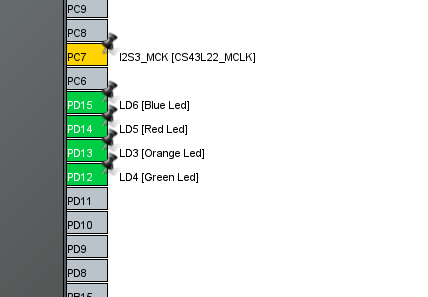
\includegraphics[width=0.85\textwidth]{Pines/leds.png}
\captionof{figure}{Configuración de pines PD12--PD15 para los LEDs integrados del STM32F407G-DISC1.}
\end{center}

\subsubsection{Pin para el Pulsador de Usuario}

El pulsador de usuario en la placa (USER BUTTON) se encuentra conectado al pin \textbf{PA0}. Este se configura como una \textbf{Interrupción externa (EXTI0)} que permite detectar los flancos de subida cuando el botón es presionado.

\begin{itemize}
\item \textbf{PA0}: GPIO External Interrupt, Rising Edge.
\end{itemize}

Además, es necesario habilitar en la pestaña \textbf{NVIC} la interrupción correspondiente a \textbf{EXTI0} para que pueda ser manejada desde el código generado.

\begin{center}
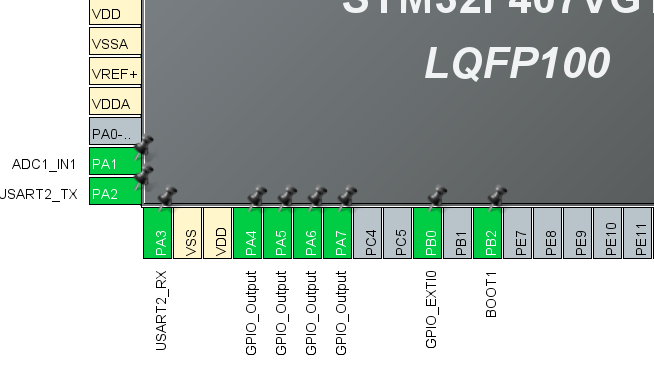
\includegraphics[width=0.75\textwidth]{Pines/pulsante.png}
\captionof{figure}{Configuración del pin PA0 como interrupción externa para el pulsador de usuario.}
\end{center}

\subsubsection{Pines para el UART2}

El periférico \textbf{USART2} se utiliza para la comunicación serie con la PC, permitiendo la visualización de mensajes y depuración a través del puerto virtual (VCP). Los pines asignados por defecto en la tarjeta STM32F407G-DISC1 son:

\begin{itemize}
\item \textbf{PA2}: USART2\_TX (Transmisión)
\item \textbf{PA3}: USART2\_RX (Recepción)
\end{itemize}

Configuración recomendada para el UART2:
\begin{itemize}
\item Baud Rate: 115200 bps.
\item Word Length: 8 Bits.
\item Stop Bits: 1.
\item Parity: None.
\item Mode: TX/RX.
\end{itemize}

\begin{center}
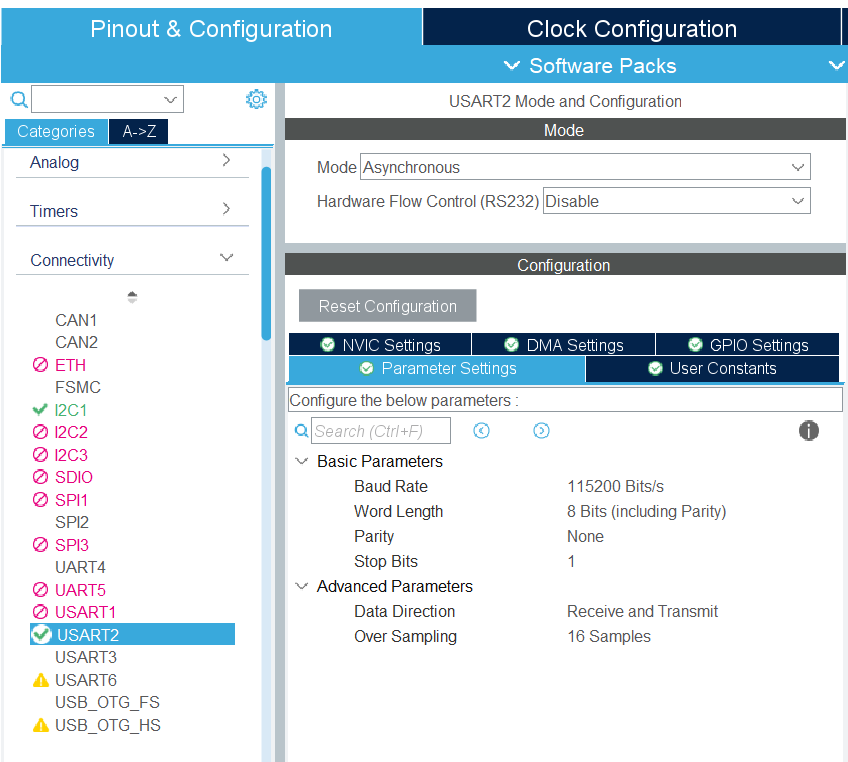
\includegraphics[width=0.8\textwidth]{Pines/uart2.png}
\captionof{figure}{Configuración del periférico UART2 en CubeMX.}
\end{center}

\subsection{Configuración de FreeRTOS en CubeMX}

Para gestionar tareas concurrentes dentro del proyecto, se activa el sistema operativo en tiempo real \textbf{FreeRTOS}. Esta configuración se realiza en la pestaña \textbf{Middleware > FREERTOS}.

\subsubsection{Tareas definidas en el código}



\begin{itemize} 
\item \textbf{defaultTask} — Handler: \texttt{StartDefaultTask} — \textbf{Prioridad: osPriorityAboveNormal}.
Descripción: tarea de prioridad "media" que alterna el LED naranja (PD13) y emite por UART el mensaje "Tarea Media ejecutada" cada 500 ms. 
\item \textbf{TareaBaja} — Handler: \texttt{StartTareaBaja} — \textbf{Prioridad: osPriorityLow}.
Descripción: tarea de baja prioridad que alterna el LED verde (PD12) cada 1000 ms. 
\item \textbf{TareaAlta} — Handler: StartTareaAlta — Prioridad: osPriorityHigh.
Descripción: tarea de alta prioridad que controla el LED rojo (PD14) en función de la variable global volátil \texttt{led\_rojo\_activado}. Si \texttt{led\_rojo\_activado} es 1, enciende el LED durante 2000 ms; si es 0 apaga el LED y espera 500 ms.
\end{itemize}

En el ioc se generan las tareas, sin embargo su funcionalidad se genera en el código por lo que de manera visual solo se crea el espacio para su posterior programación.




\begin{center}
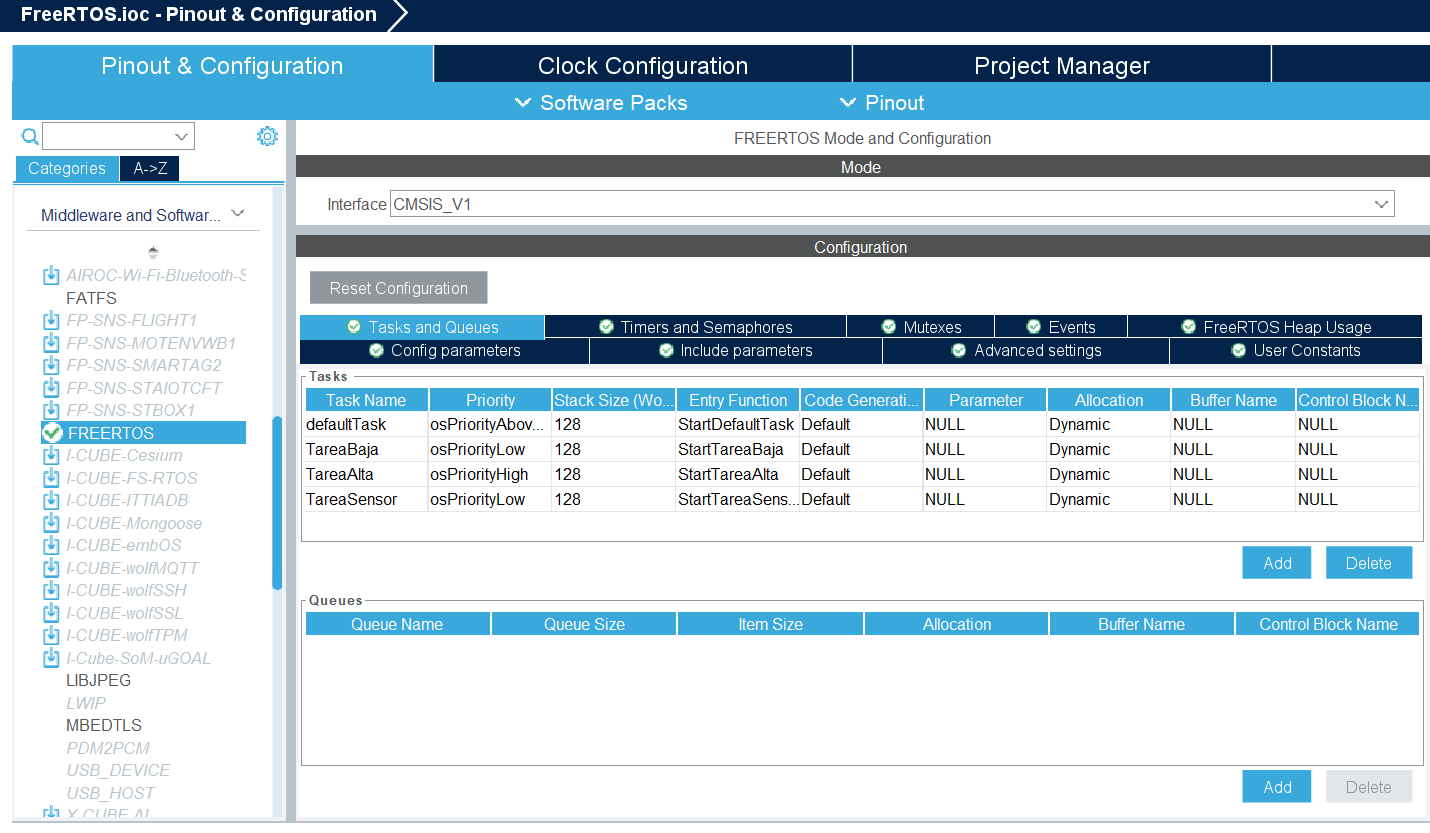
\includegraphics[width=0.85\textwidth]{Pines/rtos.png}
\captionof{figure}{Configuración de tareas y prioridades en FreeRTOS desde STM32CubeMX.}
\end{center}

\section{Resultados}

Una vez configurados los pines, periféricos y tareas en FreeRTOS, se procedió a cargar el programa en la placa de desarrollo \textbf{STM32F407G-DISC1}.  
El objetivo de esta fase fue comprobar el funcionamiento concurrente de las tareas, la correcta lectura del pulsador y la transmisión de datos por UART.

\subsection{Comprobación de la ejecución de tareas}

Durante la ejecución se observó que las tres tareas del sistema (alta, baja y por defecto) operan de forma simultánea bajo la planificación de FreeRTOS:

\begin{itemize}
    \item La tarea \textbf{TareaAlta} (prioridad alta) controla el LED rojo (PD14) según el estado de la variable global modificada en la interrupción externa.
    \item La tarea \textbf{defaultTask} (prioridad normal) realiza el parpadeo del LED naranja (PD13) y envía mensajes periódicos por el puerto UART2.
    \item La tarea \textbf{TareaBaja} (prioridad baja) controla el LED verde (PD12) con una frecuencia de parpadeo más lenta.
\end{itemize}

En la siguiente figura se observa la placa durante la ejecución, con los tres LEDs funcionando de manera independiente.

\begin{center}
    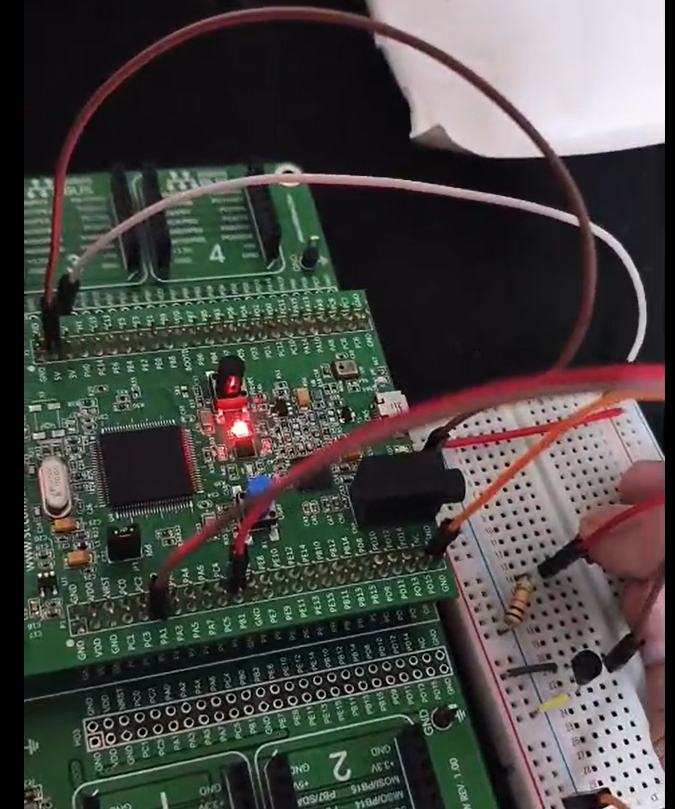
\includegraphics[width=0.8\textwidth]{Resultados/result.png}
    \captionof{figure}{Ejecución de las tareas: LEDs parpadeando de manera concurrente bajo FreeRTOS.}
\end{center}


\subsection{Comunicación por UART2}

La comunicación serial a través de \textbf{USART2} permitió verificar el comportamiento de las tareas mediante mensajes enviados al monitor serie (velocidad de 115200 baudios).  
Cada 500 ms, la tarea principal imprime el estado del sistema, demostrando que FreeRTOS mantiene una temporización estable.

\begin{center}
    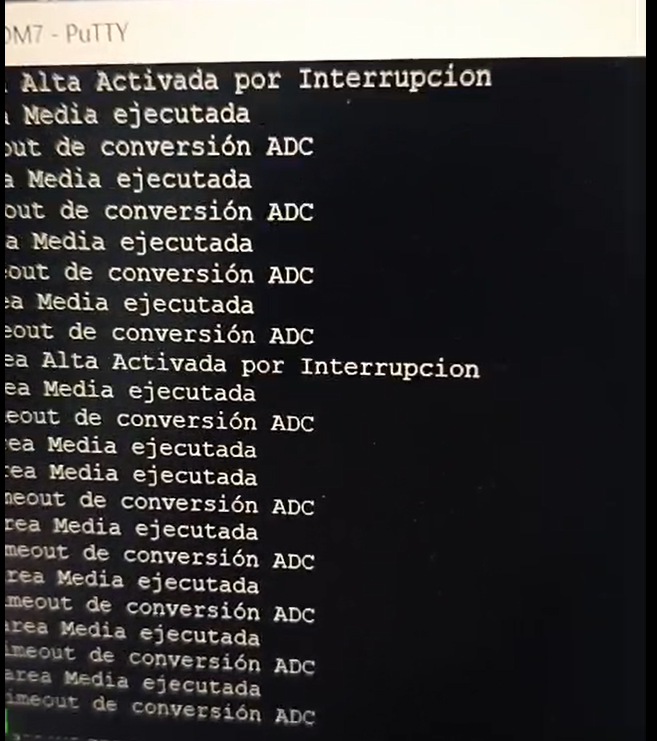
\includegraphics[width=0.9\textwidth]{Resultados/putty.png}
    \captionof{figure}{Mensajes enviados por UART2 durante la ejecución del programa.}
\end{center}




\end{document}
